\mode<presentation>
{
  \usetheme{CambridgeUS}
  \usecolortheme{whale}
  \usecolortheme{lily}

  \setbeamercovered{transparent}
  \usefonttheme[onlymath]{serif}
}

\title[\IntroduceCourseMaterialShortName] % (optional, use only with long paper titles)
{\course: \IntroduceCourseMaterialName\license}

\subtitle
{Lecture \IntroduceCourseMaterialNumber} % (optional)



\begin{document}

\begin{frame}
  \titlepage
\end{frame}

\mode<article>{
\maketitle
\tableofcontents
}

\section{Motivation for the Course}

Feedback control systems can be found practically everywhere these days. Some are very simple, such as the float controller for the water level in your toilet tank. Others are extremely complicated, such as the many control systems used by a modern jet airplane. In fact, modern feedback control theory and practice largely co-evolved with the aerospace industry. You'll find feedback control concepts taught in multiple departments at many universities, especially in Electrical, Mechanical, Aerospace, and Chemical Engineering programs.

Feedback controllers can be useful in solving a wide variety of real-world problems. One common example in the news these days is autonomous vehicles. This video \url{https://www.youtube.com/watch?v=cdgQpa1pUUE} gives an early example from 2012 of a self-driving car and how it can enhance the quality of life for a person who is legally blind. Of course, we would be remiss to avoid pointing out that autonomous vehicles have also been in the news lately with negative outcomes like accidents, even resulting in death. Like most engineered systems, they are far from perfect, which is a good reminder for all of us engineers to think about the consequences of our engineering design decisions, both in terms of how we define and how we solve problems. 

\begin{frame}{Feedback Control Overview}
	Let's take a look at a feedback control system for a set of solar panels tracking the sun as it moves across the sky: 
\begin{center}
		\url{https://www.youtube.com/watch?v=bE179wgm164} \\
%	\includegraphics[height=1in]{\mainfolder/Control_System_of_the_Week/Smart_Grids/"512px-Giant_photovoltaic_array.jpg} \\
\end{center}
\end{frame}
How do these concepts connect with what we'll learn this semester? Compare the video to the schedule at the end of the Syllabus and you'll see that...

\begin{itemize}
\setlength\itemsep{0pt}
\setlength\parskip{0pt}
	\item you'll learn the basic principles of modeling -- meaning creating differential equation or Laplace-domain representations for -- physical systems starting in Lecture \ModelingMechanicalSystemsNumber: \ModelingMechanicalSystemsName.
	\item we'll do a quick review of some differential equation concepts that will remind you of the connection between an integral and the Laplace-domain function $\frac{1}{s}$ in Lecture \LaplaceTransformReviewNumber: \LaplaceTransformReviewName. 
	\item we'll talk more about using Simulink to model systems in Lecture \IntroToSimulinkNumber: \IntroToSimulinkName
	\item you'll learn more about the block diagram representation that is used in Simulink in Lecture \BlockDiagramsNumber: \BlockDiagramsName. 
	\item we'll design closed-loop feedback controllers in a number of lectures, starting with Lecture \ControlAndStabilityNumber: \ControlAndStabilityName.
	\item you'll learn specifically about modeling rotational mechanical systems (like the solar panels) in Lecture \RotationalAndFluidSystemsNumber: \RotationalAndFluidSystemsName. 
	\item you'll learn how to model DC motors in Lecture \MotorModelingNumber: \MotorModelingName. 
	\item and more!	
\end{itemize}



\begin{frame}{Some definitions}
The subject of this course is {\color{green}feedback control} of {\color{red}dynamic} {\color{cyan}systems}.
\end{frame} These color-coded terms are defined in the next couple of pages. 
\begin{frame}{What are systems?}
\begin{itemize}
\item A {\color{cyan}system} is an interconnected subset of the universe!
\item Example Systems:
\end{itemize}
\begin{center}
\includegraphics[width=8cm]{figures/examplesystems}
\end{center}
\end{frame}
In this class, we will represent systems using blocks.
\begin{center}
	\includegraphics[width=2cm]{figures/systemalone}
\end{center}

\begin{frame}{Input and Output \em Signals}
\begin{itemize}
\item By definition, we have to separate a system from the rest of the world
\begin{itemize}
\item Input signals: connection variables that we will determine
\item Output signals: connection variables that we will observe, whether by predicting (using mathematical models) or measuring
\end{itemize}
\end{itemize}
\begin{center}
\includegraphics[width=5cm]{figures/system}
\end{center}
\end{frame}
Signals are represented by arrows.
\begin{center}
	\includegraphics[width=2cm]{figures/signalalone}
\end{center}

It can be useful to categorize systems as either \textit{static} or \textit{dynamic}.
\begin{frame}{Static vs. Dynamic Systems}
\begin{itemize}
\item Static System
\mode<article>{
\begin{center}
	\includegraphics[width=1.5cm]{figures/switch}
	\hspace{1in}
	\includegraphics[width=5cm]{figures/staticsystem}
\end{center}
}
\mode<presentation>{
\begin{columns}
\begin{column}{2cm}
\begin{center}
\includegraphics[width=1.5cm]{figures/switch}
\end{center}
\end{column}
\begin{column}{5cm}
\includegraphics[width=5cm]{figures/staticsystem}
\end{column}
\end{columns}
}
\item {\color{red}Dynamic} System
\mode<article>{
	\begin{center}
		\includegraphics[width=2cm]{figures/car}
		\hspace{1in}
		\includegraphics[width=5cm]{figures/dynamicsystem}
	\end{center}
}
\mode<presentation>{
\begin{columns}
\begin{column}{2cm}
\begin{center}
\includegraphics[width=2cm]{figures/car}
\end{center}
\end{column}
\begin{column}{5cm}
\includegraphics[width=5cm]{figures/dynamicsystem}
\end{column}
\end{columns}
}
\item What is the difference?
\end{itemize}
\end{frame}
A static system does not depend on the state of the system at previous times. In other words, the light will be on whenever the light switch is in the position corresponding to ``on'' (usually up), no matter whether it has been on or off in the past. A dynamic system, however, does depend on the state of the system in the past. In the car example, if the car starts at 0 mph, a given throttle position will result in a slower speed 3 seconds later than that same throttle position for a car that is already moving at 30 mph. 

In this class, we will primarily concern ourselves with dynamic systems. We will create mathematical models of these systems using differential equations (time domain) or Laplace-domain equations. 


\begin{frame}{Open vs. Closed-Loop Control Systems}
\begin{itemize}
\item Open Loop System
\begin{center}
\includegraphics[width=6cm]{figures/openloopcontrol}
\end{center}
\item Closed Loop Control ({\color{green}Feedback Control})
\begin{center}
\includegraphics[width=8.415cm]{figures/closedloopcontrol}
\end{center}
\end{itemize}
\end{frame}

An open-loop control system is one in which you must determine the input signal (arrow going in to the ``Actuator'' block in the first example above) ahead of time to achieve a desired output signal (arrow coming out of the ``System'' block). Open loop control is usually ineffective for anything but the simplest systems. It requires you to know the system and actuators perfectly and that there be no unexpected disturbances.

A closed-loop system is one in which you can start at any point along the system, traveling through the systems (blocks) and signals (arrows) until you reach your starting point again. Closed-loop control can be very effective since it relies on a measurement (arrow coming out of the ``Sensor'' block) of the output signal (arrow connecting the ``System'' and ``Sensor'' blocks), which the controller uses to determine the input signal to the actuator. Feedback control can correct for a wide variety of problems and is a key focus of this class. 

% KEJ Note: ofen example was moved to "Quiz Yourself"
%\begin{frame}{Example of Open or Closed Loop Control?}
%\begin{itemize}
%\item What kind of control systems are used here?
%\begin{center}
%\includegraphics[width=4cm]{figures/oven}
%\end{center}
%\end{itemize}
%\end{frame}
\begin{frame}{Feedback Control Elements}
%\begin{minipage}{2.5in}\begin{center}
%Identify the block elements for a two-wheeled robot
%\end{center}
%\end{minipage}
%\begin{minipage}{2in}\begin{center}
%\includegraphics[height=1.25in]{figures/aerospace}
%\end{center}\end{minipage}\\
\begin{center}
\includegraphics[height=1.5in]{figures/closedloopcontrol}
\end{center}
\end{frame}

The elements in the feedback control loop include

\begin{itemize}
	\setlength\itemsep{0pt}
	\setlength\parskip{0pt}
	\item the ``System", often called the ``Plant'' or ``Plant System'', which is whatever you are trying to control. For example the relationship between the force generated by the engine and speed of a car can be defined as a system.
	\item the ``Sensor,'' which measures the output signal. On a car, this would be your speedometer.
	\item the ``Controller'' (labeled ``Control'' in this article), which is typically performed by a computer to determine the throttle position needed by the engine to generate the desired amount of force (or power).
	\item the ``Actuator,'' which in this car example would be the relationship from the throttle position to the engine's force (or power). In this class, we will usually not consider the actuator separately from the plant system but will instead combine them assuming a perfect actuator. 
\end{itemize}


%}



%\section{\textcolor{red}{Section Heading}}
%
%\textcolor{red}{I (Katie) created these files as a template for creating new lecture articles and presentations (with homework and quiz yourself problems) in Fall 2022. The folder can be copied as a whole and then new content added.}
%
%
%\begin{frame}{\textcolor{red}{Frame Content for Presentation File}}
%\begin{center}
%\mode<article>{\includegraphics[width=4.5in]{figures/emptyfig.png}
}
%\mode<presentation>{\resizebox{3in}{!}{\includegraphics[width=4.5in]{figures/emptyfig.png}
}}
%\end{center}
%\end{frame}


%\section{Application Example}
%
%\textcolor{red}{Application example goes here, if one exists.}


\section{Lecture Highlights}
The primary takeaways from this article include
\begin{enumerate}
\setlength{\itemsep}{5pt}
\setlength{\parskip}{0pt}
\setlength{\parsep}{0pt}
\item Feedback control impacts many aspects of our modern lives and is important to a number of engineering disciplines.
\item We'll be working with both signals (represented by arrows, sometimes called variables) and systems (represented by boxes) in this class.
\item Control is most effective when it is configured in feedback (closed-loop), which allows for things like imperfect models and disturbance inputs. However, we'll still need to develop mathematical models for open-loop plant systems in this class so that we can use these to build the best controllers.
\end{enumerate}

\section{Quiz Yourself}

\subsection{Questions}
\begin{enumerate}
\setlength{\itemsep}{5pt}
\setlength{\parskip}{0pt}
\setlength{\parsep}{0pt}
\item \input{quizfigures/quizyourself1.tex} 
\item True or false: the figure below is of a closed-loop (feedback) system. \\
\begin{center} 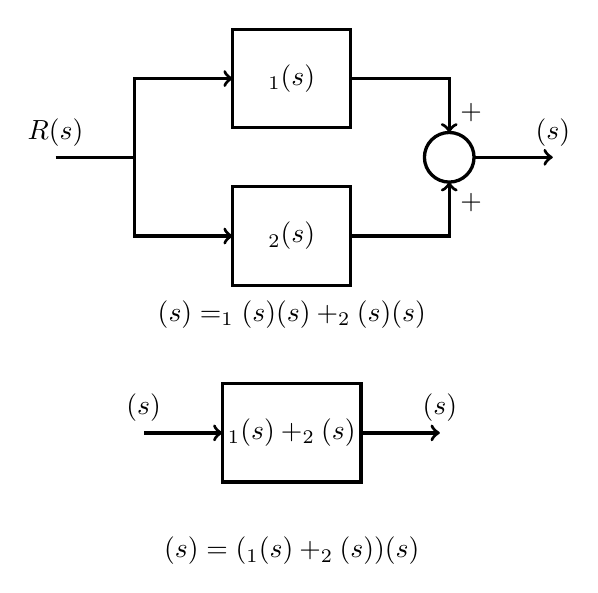
\begin{tikzpicture}[inner sep=0pt,outer sep=0pt,very thick,
sysblock/.style={draw,rectangle,inner sep=2pt,minimum width=1.5cm,minimum height=1.25cm,very thick}]
\draw (1,1) node[sysblock] (G1) {$\plant_{1}(s)$};
\draw (1,-1) node[sysblock] (G2) {$\plant_{2}(s)$};
\draw (-2,0) node[above=4pt] {$R(s)$} -- (-1,0);
\draw[->] (-1,0) |- (G1.180);
\draw[->] (-1,0) |- (G2.180);
\draw (3,0) node[draw,circle] (sum) {$\rule{0pt}{18pt}$};
\draw[->] (G1.0) -| (sum.90) node[above right=4pt] {$+$};
\draw[->] (G2.0) -| (sum.-90) node[below right=4pt] {$+$};
\draw[->] (sum.0) -- ++(1,0) node[above=4pt] {$\outptLT(s)$};
\draw (1,-2) node {$\outptLT(s)=\plant_{1}(s)\inptLT(s) + \plant_{2}(s)\inptLT(s)$};

\draw (1,-3.5) node[sysblock] (GG) {$\plant_{1}(s)+\plant_{2}(s)$};
\draw[<-] (GG.180) -- ++(-1,0) node[above=4pt] {$\inptLT(s)$};
\draw[->] (GG.0) -- ++(1,0) node[above=4pt] {$\outptLT(s)$};
\draw (1,-5) node {$\boxed{\outptLT(s)=(\plant_{1}(s)+\plant_{2}(s))\inptLT(s)}$};

\end{tikzpicture}
 \end{center}
\item In a human body, the normal temperature fluctuates around 37 °C, but many factors can affect this, e.g., diseases, hormones, etc. These factors could lead to a low or high temperature. The temperature regulation process is controlled by human brain. Sketch and label the signals (arrows) and system(s) (block(s)) involved in the process of regulating human body temperature. Make it clear to the reader what dose each block represents.
\end{enumerate}

\subsection{Solutions}

\begin{enumerate}
\setlength{\itemsep}{5pt}
\setlength{\parskip}{0pt}
\setlength{\parsep}{0pt}
\item The stovetop burners typically use \textit{open loop} control: you set the burner knob to your desired setting, and the burners heat up accordingly. (Some people would call this a ``human-in-the-loop" controller because you might turn the knob up or down depending on how your cooking is going.) The oven is typically a closed-loop control system because a thermometer inside the oven measures the oven's temperature and automatically turns the oven heater on or off to maintain the desired temperature. 
\item False. Although two branches exist, if you start on any arrow in this system and follow the arrow directions through the systems and summing block you will end up at the output signal, not back at the arrow where you started. This is actually an example of a parallel system, which we will study in more detail in Lecture \BlockDiagramsNumber: \BlockDiagramsName.
\item The feedback loop described is shown in the image below. \\
\begin{center}
	\includegraphics[width=4.5in]{quizfigures/quiz03soln.pdf}
\end{center} 
In the feedback loop, the \textbf{thermoreceptors} act as sensors, detecting changes in body temperature. The \textbf{hypothalamus} controls a variety of effectors that respond to the change in body temperature. There are several \textbf{effectors} that are the actuators and are controlled by the hypothalamus that can respond to body temperature change. These include blood vessels near the skin and skeletal muscles.
%\item \rule{0pt}{12pt}\\ % use this \rule command to correctly align solutions given as images
\end{enumerate}



\end{document}


